
\section{Niðurstöður}
\label{sec:nidurstodur}

Samkvæmt útreikningum okkar hefðu plöturnar gefið sig á undan boltunum eða við $4375 N$, \sbr kafla \ref{ch::reikningar}.
Boltarnir hefðu átt að þola allt að $13100 N$ álag.

\begin{figure}[h]
  \centering
  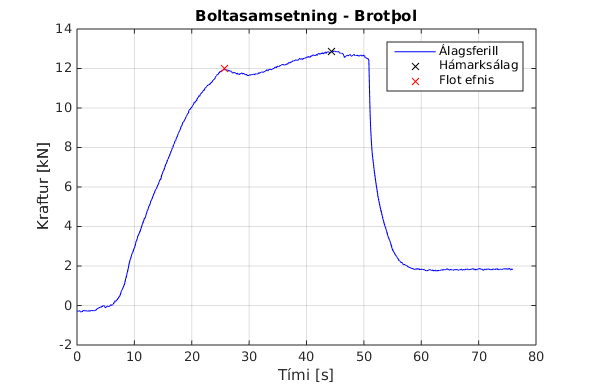
\includegraphics[width=\linewidth]{alag}
  \caption{Álagsferill í þolprófun}
  \label{fig:alag}
\end{figure}

Þar sem útreikningar okkar miðast við eina plötu, \te eftir að aðskilnaður hefur átt sér stað, er þetta ekki alveg rétt.
Ef reiknað væri með öllum plötunum, þ.e.~áður en aðskilnaður hefur átt sér stað, myndi flatartregðuvægið þrefaldast, sem passar nokkuð vel við þau gildi sem komu fram í prófunum.
Eins og sjá má á mynd \ref{fig:alag} kemst efnið í flot við \(12 kN \approx 4375 N \cdot 3 = 13.13 kN\) sem stenst nokkuð vel.
Skekkjan á því er þá \(100\% - {12 \over 13.13} = 8.61\% \)

\clearpage

\begin{figure}
  \centering
  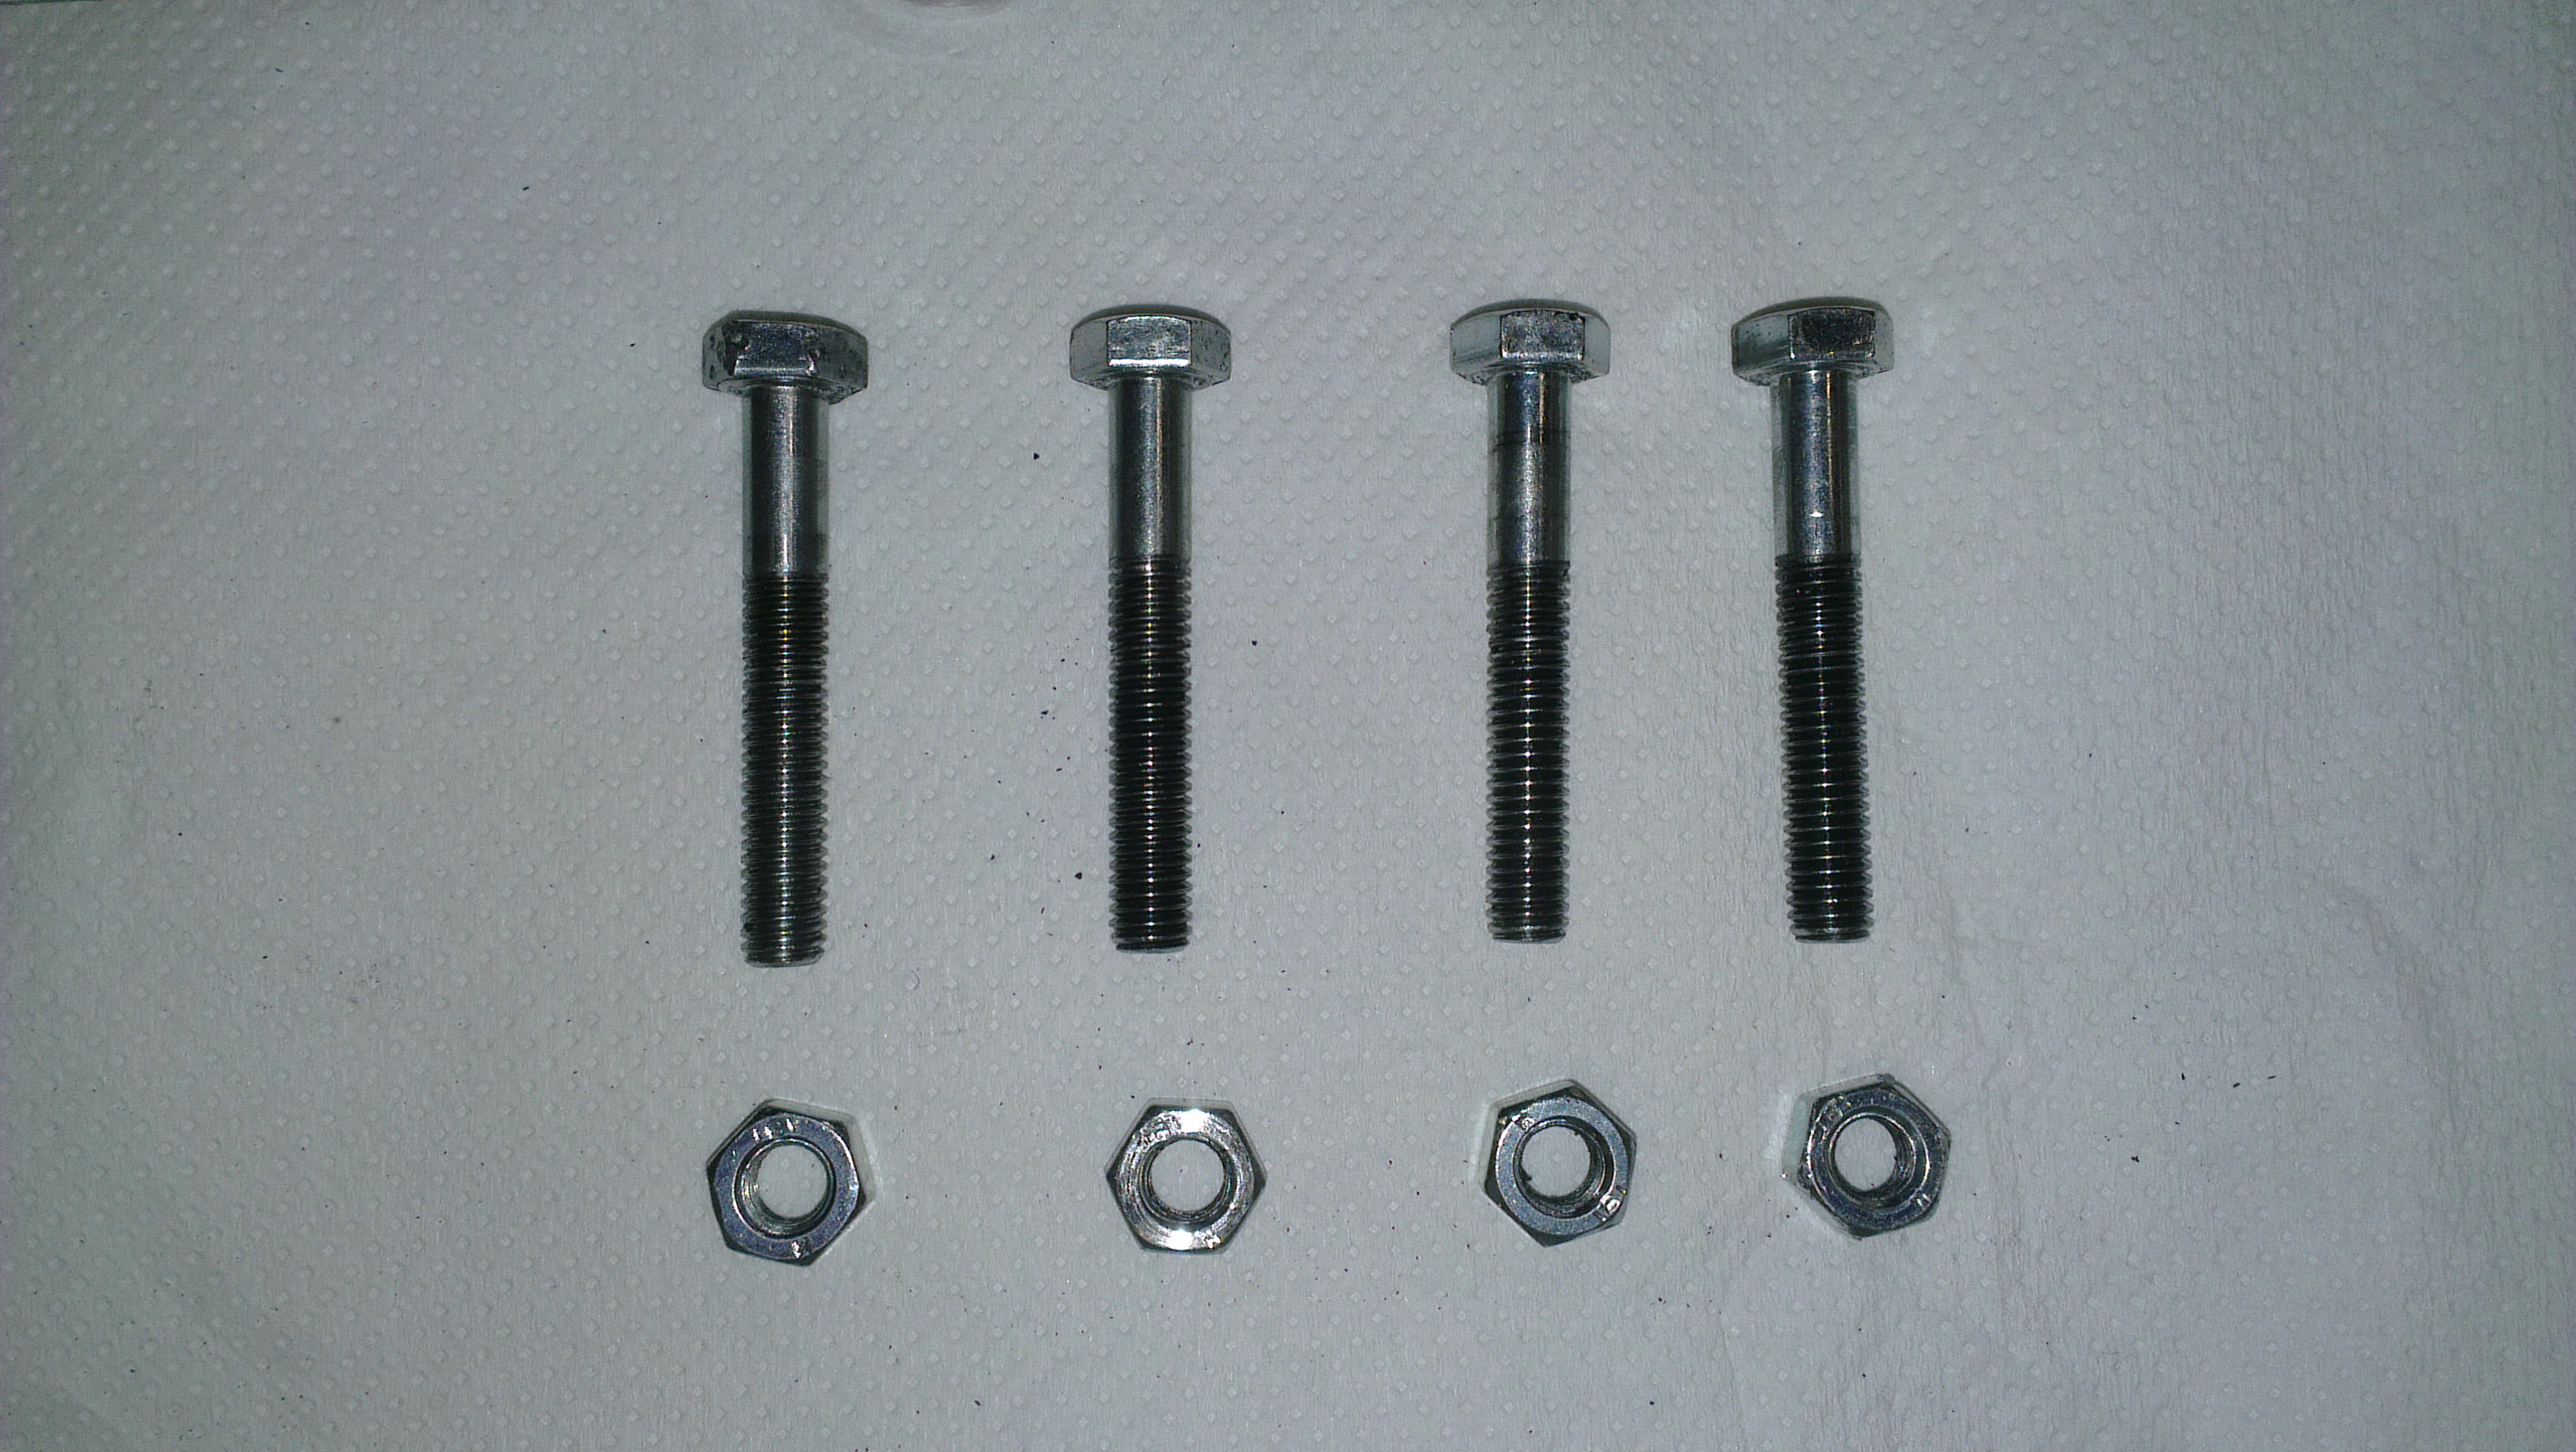
\includegraphics[width=\linewidth]{boltar}
  \caption{Boltar eftir prófun}
  \label{fig:boltar}
\end{figure}


\begin{figure}
  \centering
  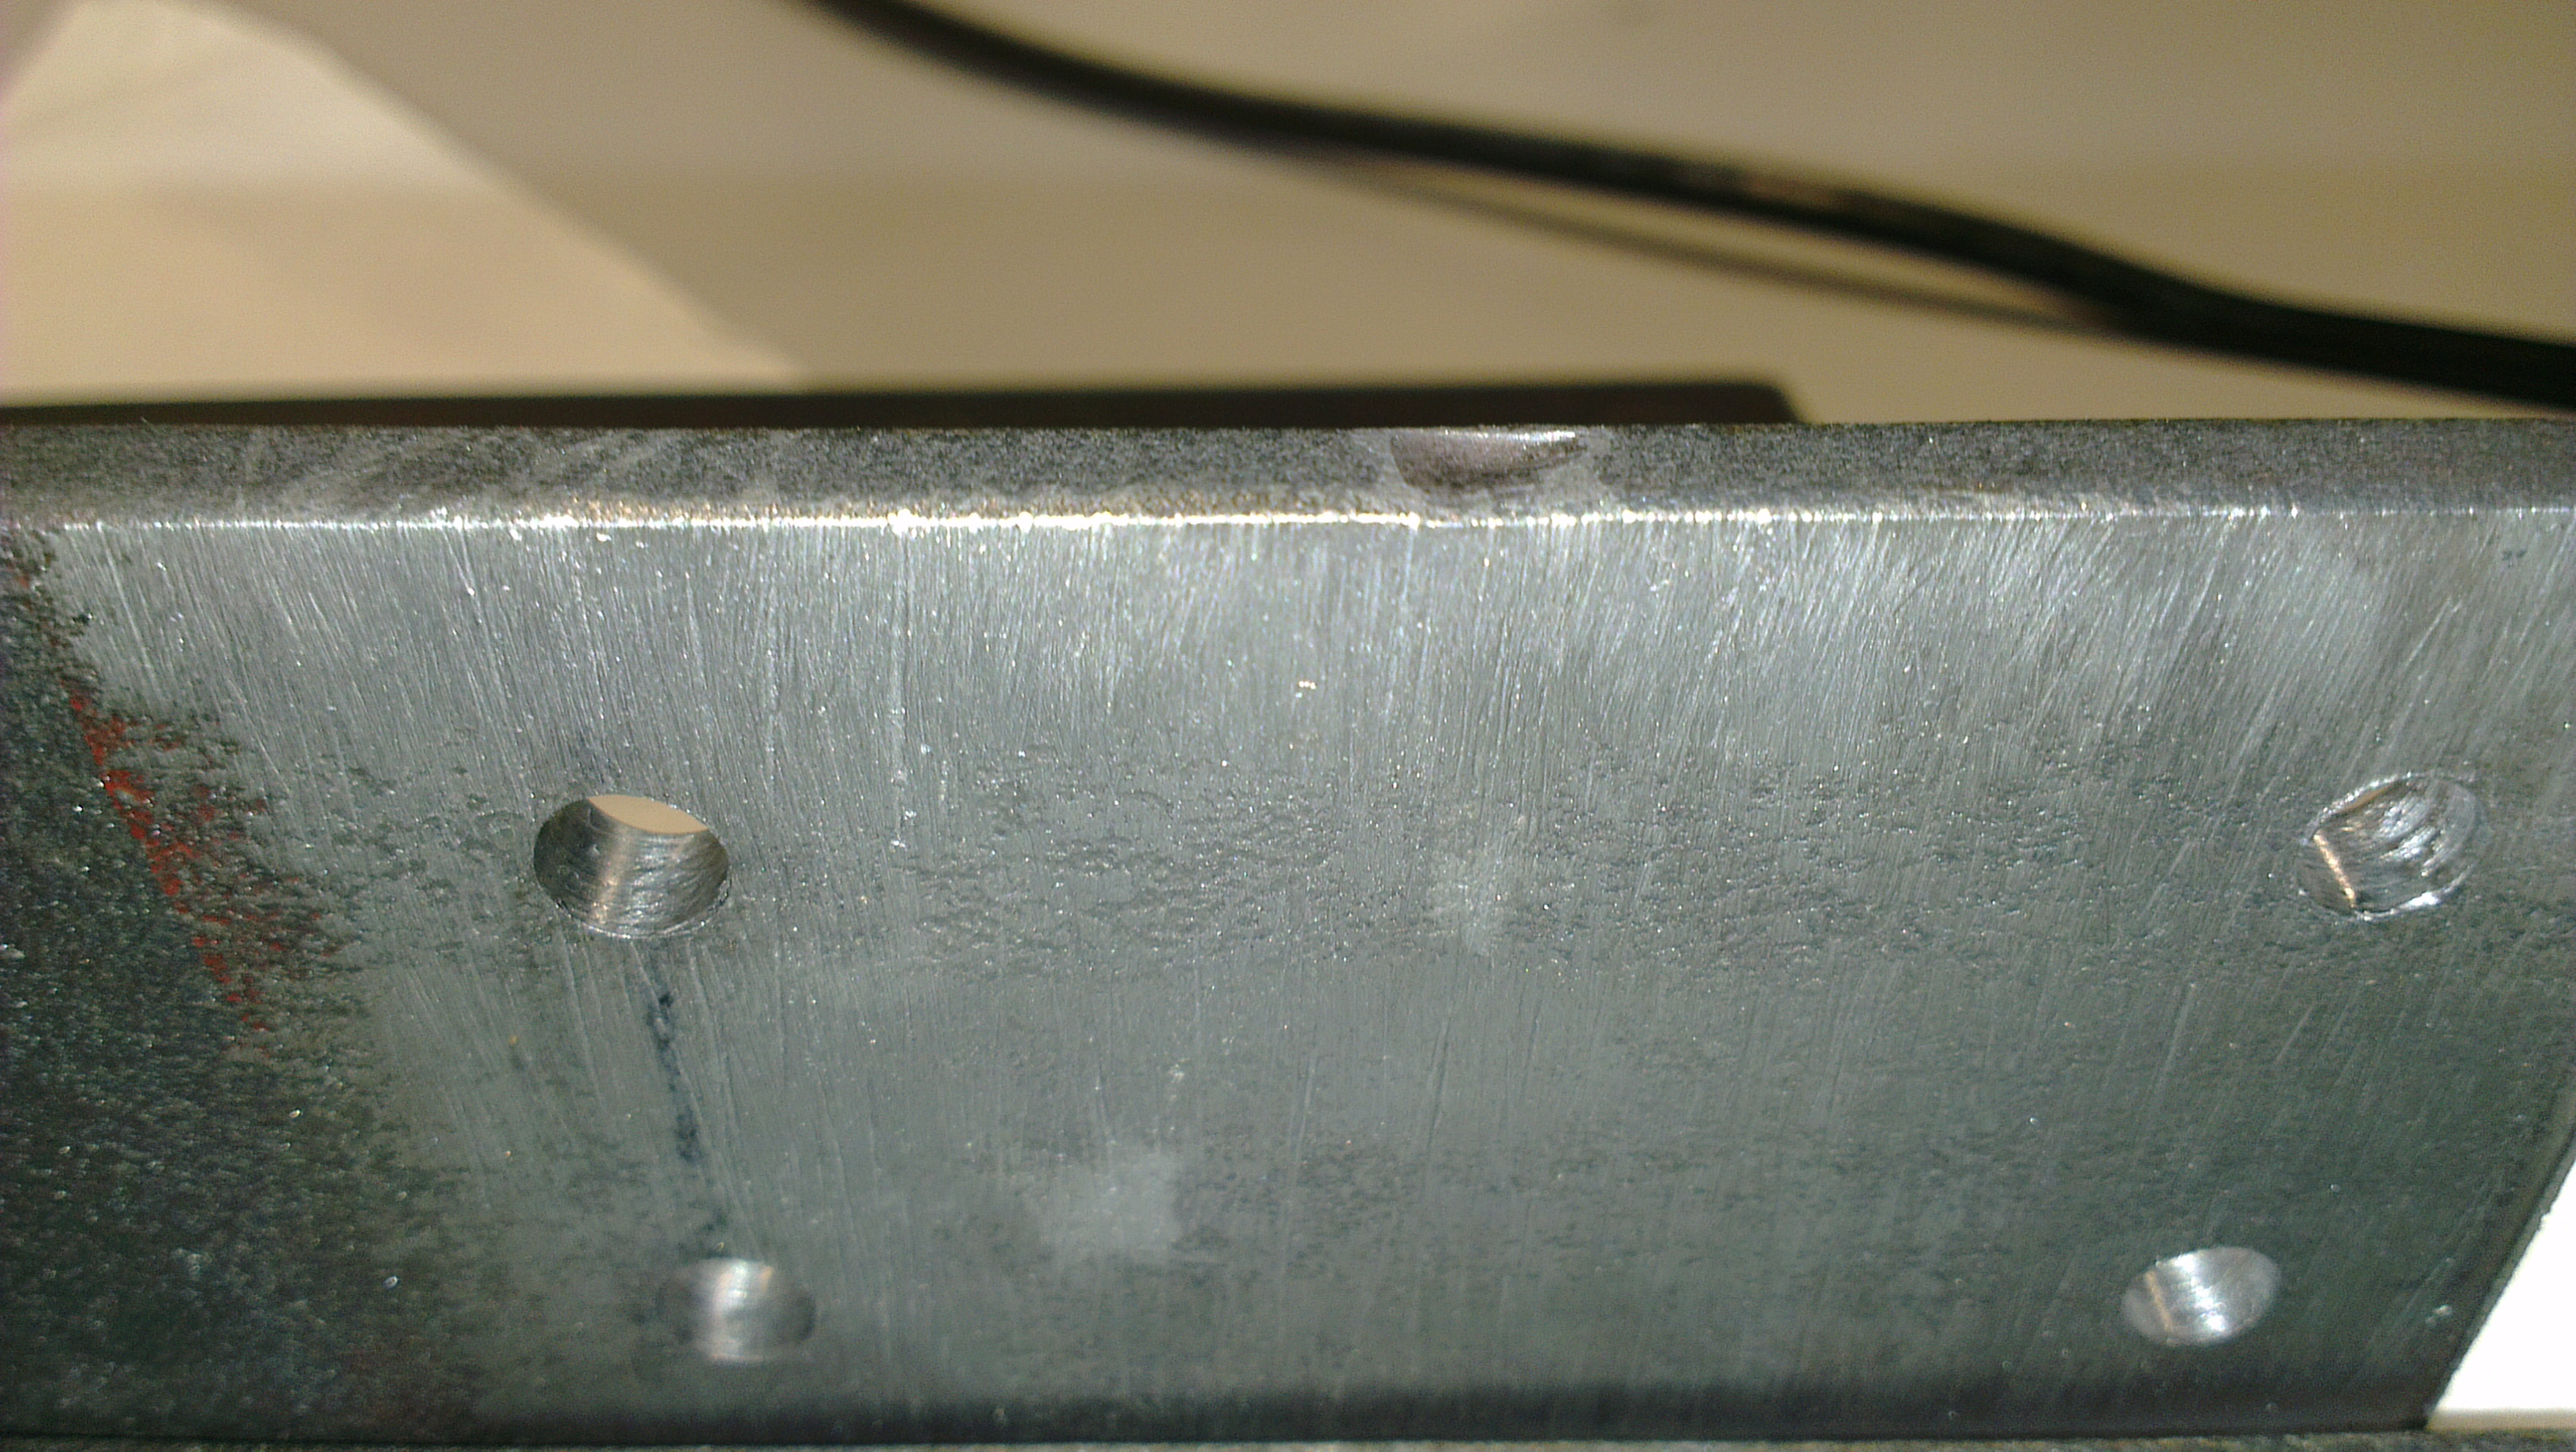
\includegraphics[width=\linewidth]{hak2}
  \caption{Hak sem myndaðist í einni stöng við prófun}
  \label{fig:hak2}
\end{figure}

\dfrac{num}{den}
\begin{figure}
  \centering
  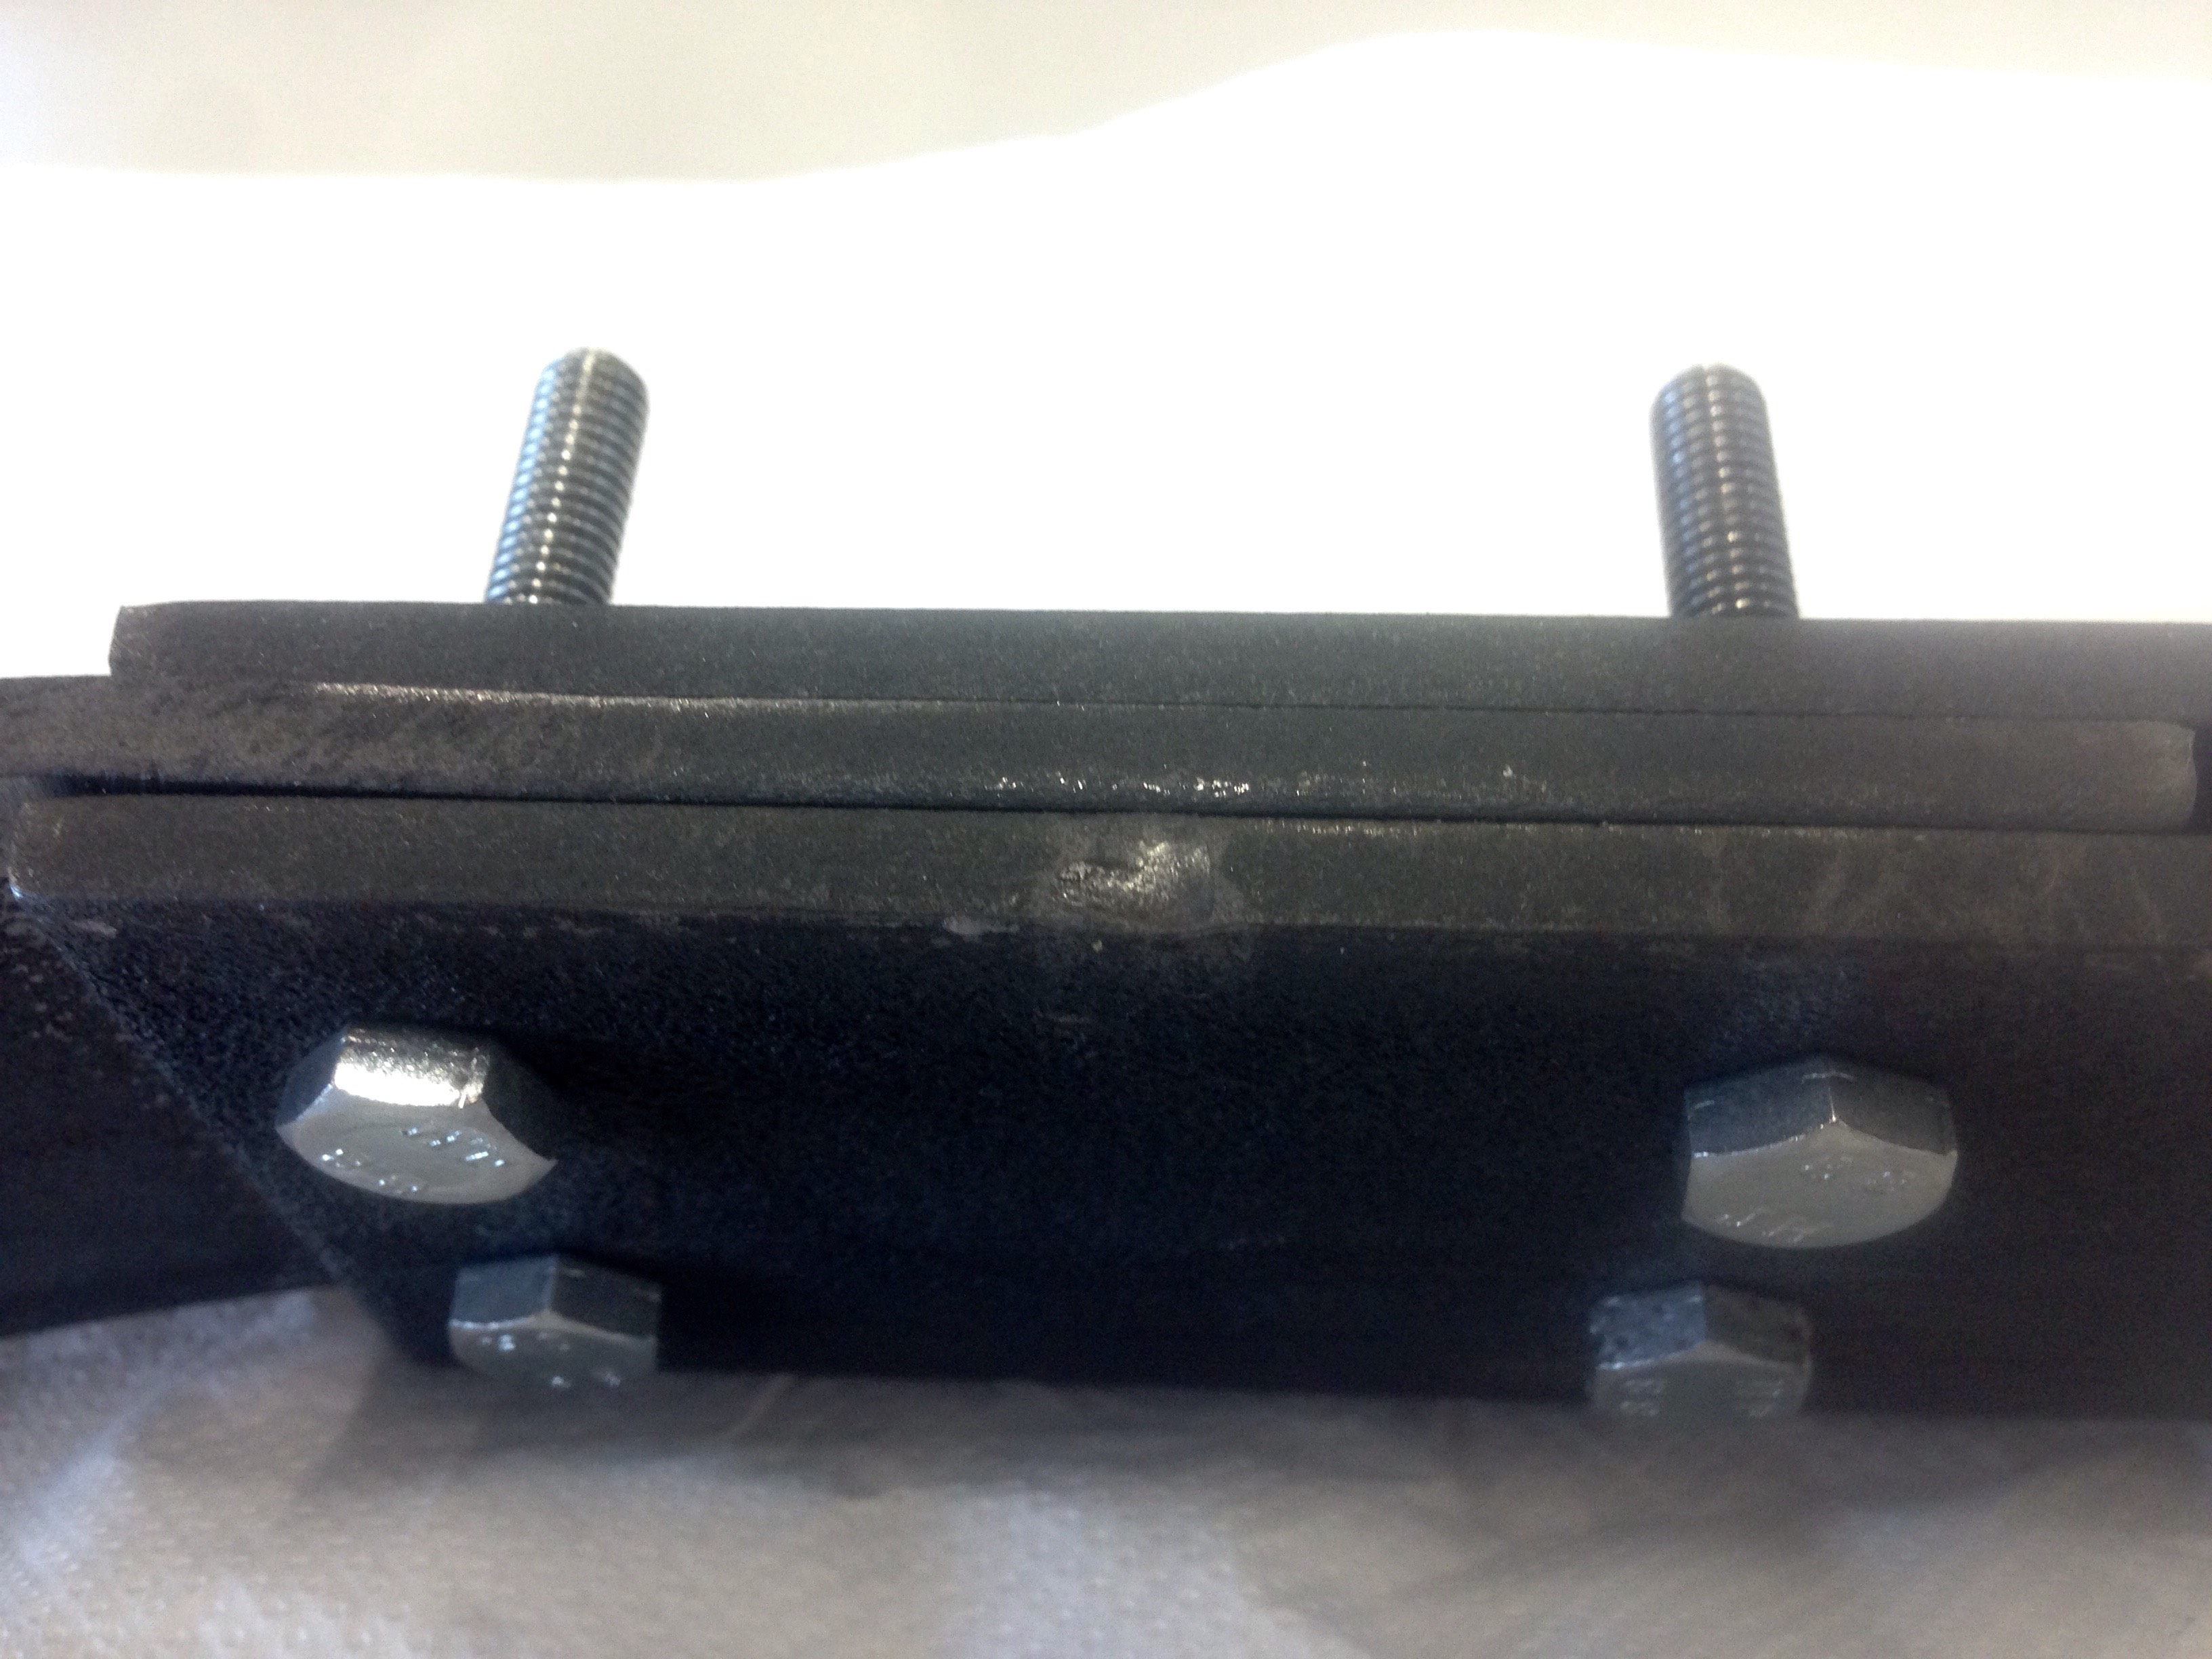
\includegraphics[width=\linewidth]{hak4}
  \caption{Hak sem myndaðist í einni stöng við prófun}
  \label{fig:hak4}
\end{figure}

Við álagsprófið beygluðust stálplöturnar en ekkert sá á boltunum, sbr. myndir \ref{fig:boltar} og \ref{fig:pano}.
Auk þess má sjá á stálplötunum að álagið var að mestu leyti á eina af ytri plötunum, sbr. myndir \ref{fig:hak2} og \ref{fig:hak4}, og því var átakið skakkt. Þetta olli því að meira af álaginu fór í stálplöturnar, en minna af álaginu í boltana.
Það olli því að plöturnar bognuður út á við áður en nægt átak færi í boltana til að valda einhverju teljanlegu átaki á boltana.

\clearpage

\begin{figure}
  \centering
  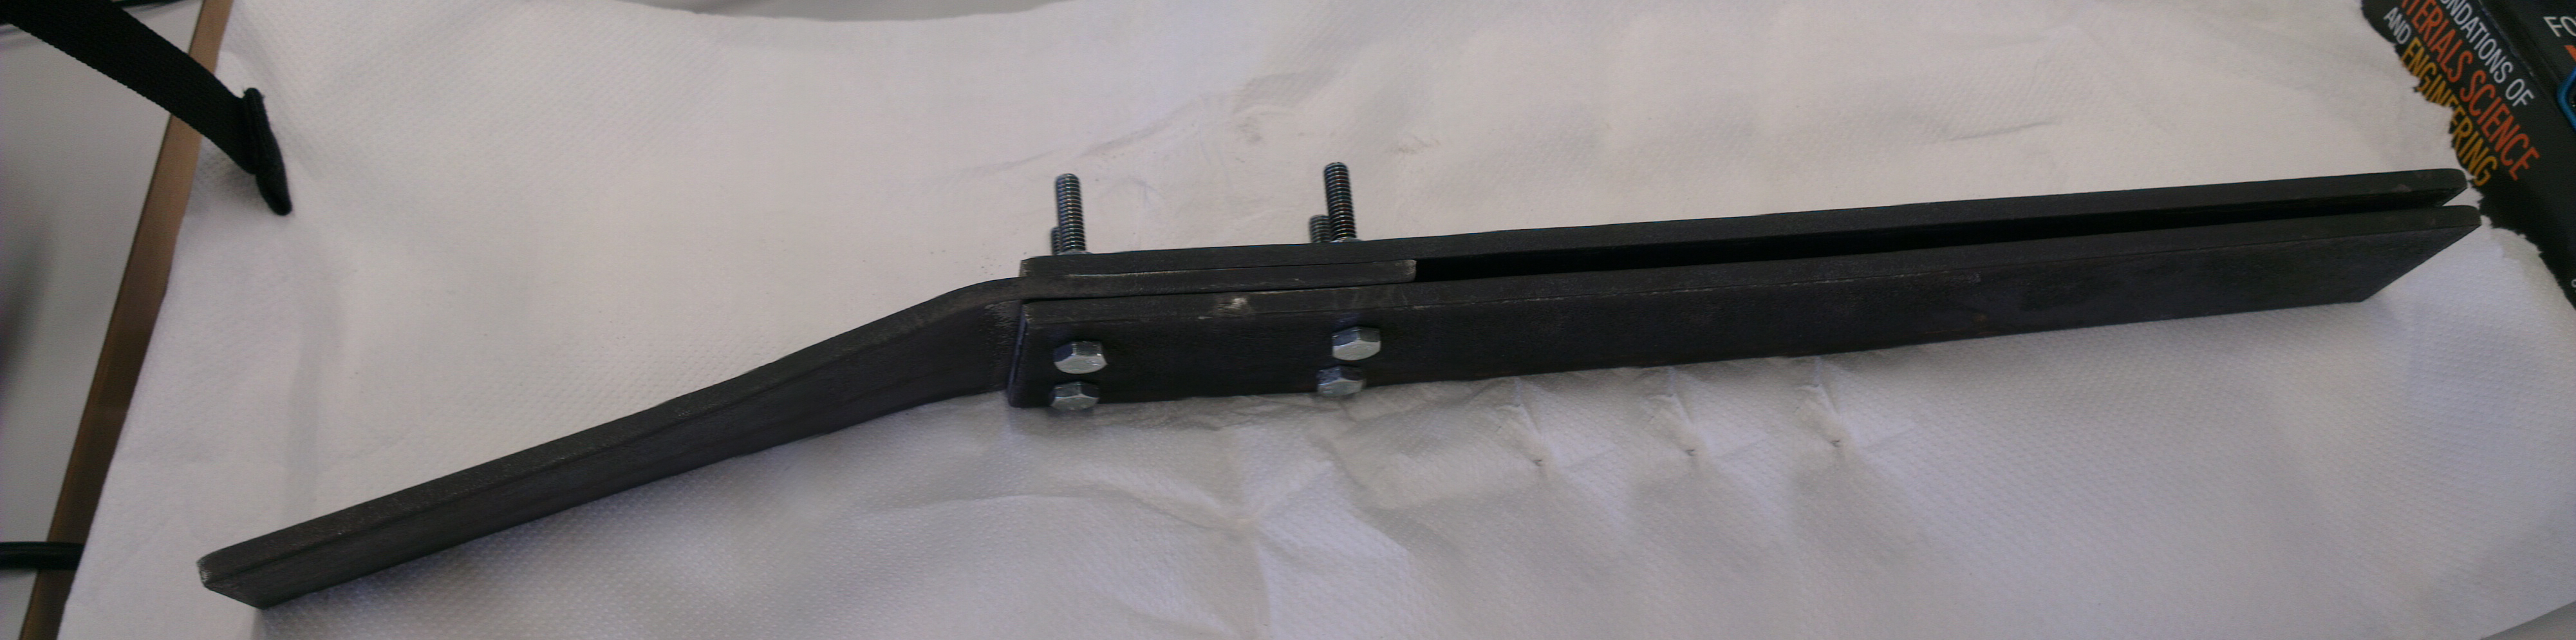
\includegraphics[width=\linewidth]{beygja_pano}
  \caption{Samsetning eftir prófun}
  \label{fig:pano}
\end{figure}


Því má í rauninni segja að prófið hafi verið gallað þar sem tækin voru ekki nógu nákvæm til að setja álagið beint ofan á plöturnar. Það olli því að plöturnar gáfu ekki eftir eins og við gerðum ráð fyrir.